\chapter{Legfontosabb eredmények}
Ebben a zárófejezetben a teljesség igénye nélkül megismétlem a legfontosabb mérési eredményeket a négy fázisból és ezeket elemzem szövegesen a teljes kép érdekében.

\section{Következtetések tanítás nélküli tesztek után kapott eredményekből.}

    \subsubsection{Összehasonlító Top-1 és Top-5 diagram a tanítás nélküli tesztekről.}
    \begin{figure}[H]
    \centering
    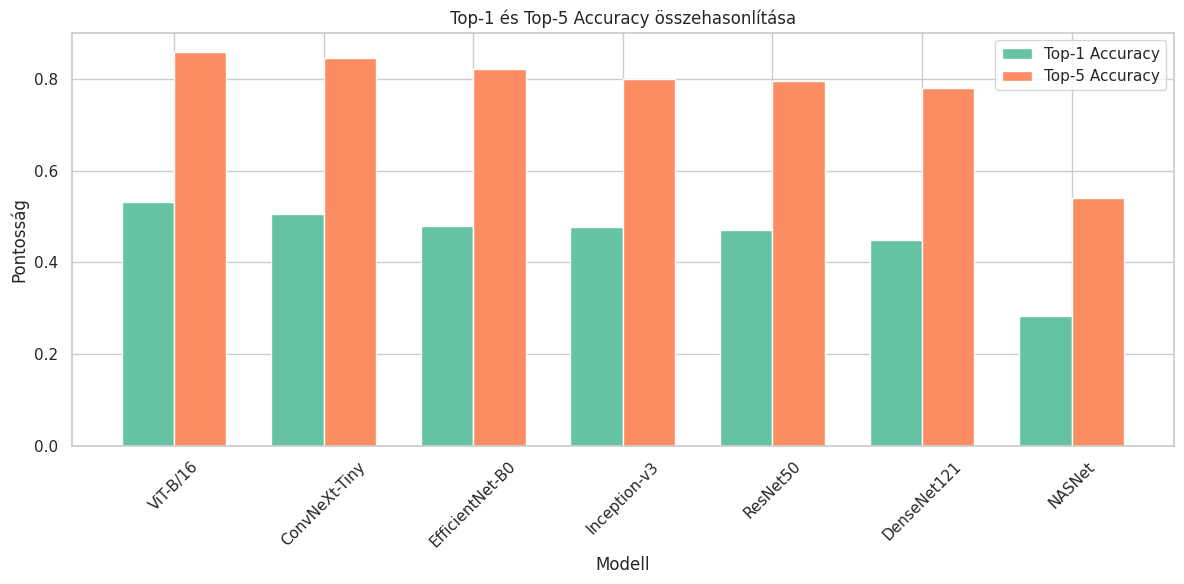
\includegraphics[width=1.0\textwidth]{images/phase01/summary01.png}
    \caption{sszehasonlító Top-1 és Top-5 diagram a tanítás nélküli tesztekről.}
    \label{fig:top1zop5phase12}
    \end{figure}

    \subsubsection{Összehasonlító Precision, Recall, F1 diagram a tanítás nélküli tesztekről.}
    \begin{figure}[H]
    \centering
    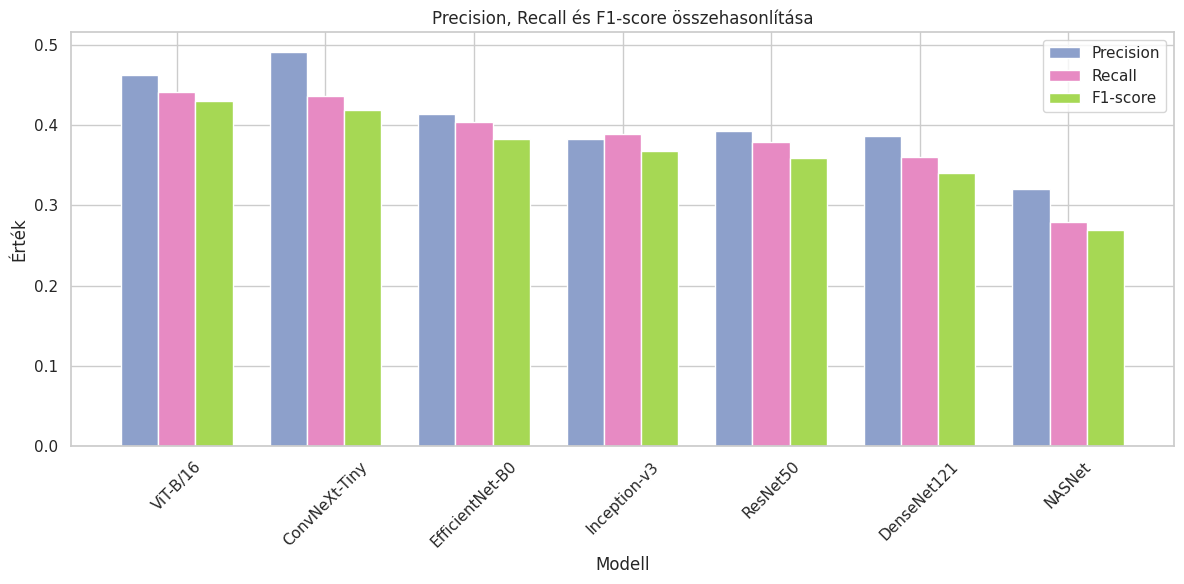
\includegraphics[width=0.75\textwidth]{images/phase01/summary02.png}
    \caption{sszehasonlító Precision, Recall, F1 diagram a tanítás nélküli tesztekről.}
    \label{fig:top1zop5phase1}
    \end{figure}

    \subsubsection{Összehasonlító idő diagram a tanítás nélküli tesztekről.}
    \begin{figure}[H]
    \centering
    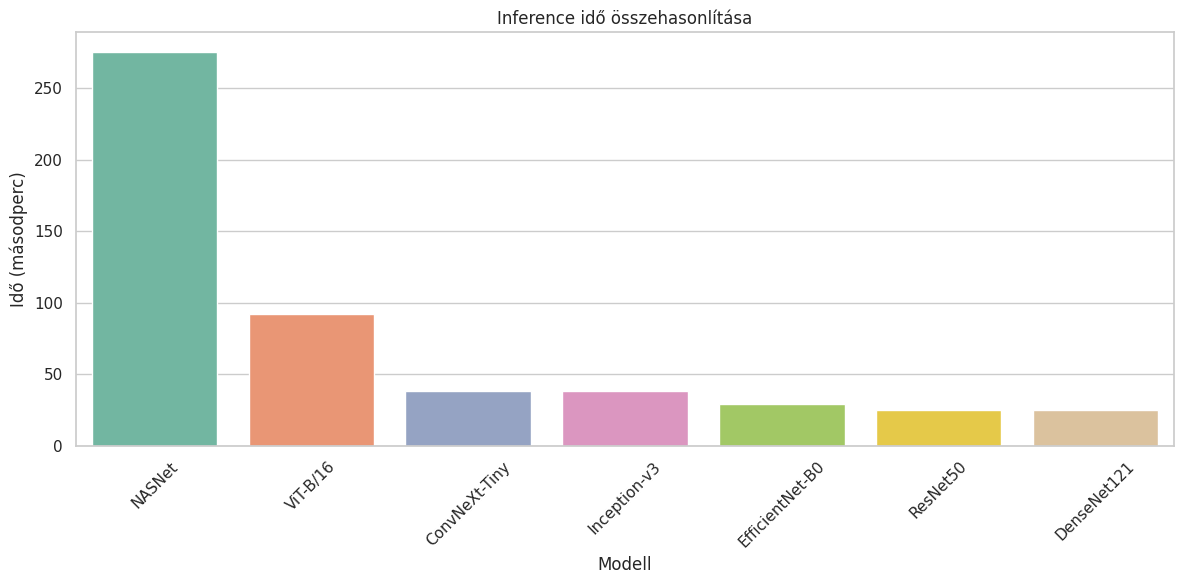
\includegraphics[width=0.75\textwidth]{images/phase01/summary03.png}
    \caption{sszehasonlító idő diagram a tanítás nélküli tesztekről.}
    \label{fig:timephase1}
    \end{figure}

    \begin{table}[H]
        \centering
        \caption{Tanítás nélküli modellek teljesítménye (Top-1 szerint csökkenő sorrendben)}
        \begin{tabular}{|l|c|c|c|c|c|c|}
        \hline
        \textbf{Modell} & \textbf{Top-1} & \textbf{Top-5} & \textbf{Prec.} & \textbf{Recall} & \textbf{F1} & \textbf{Idő (s)} \\
        \hline
        ViT-B/16 & 0.5308 & 0.8582 & 0.4629 & 0.4419 & 0.4307 & 92.13 \\
        ConvNeXt-Tiny & 0.5048 & 0.8471 & 0.4917 & 0.4369 & 0.4194 & 38.40 \\
        EfficientNet-B0 & 0.4802 & 0.8217 & 0.4137 & 0.4039 & 0.3829 & 28.89 \\
        Inception-v3 & 0.4763 & 0.8008 & 0.3833 & 0.3896 & 0.3683 & 38.06 \\
        ResNet50 & 0.4698 & 0.7962 & 0.3934 & 0.3797 & 0.3592 & 25.21 \\
        DenseNet121 & 0.4498 & 0.7806 & 0.3874 & 0.3611 & 0.3408 & 25.15 \\
        NASNet-A-Large & 0.2820 & 0.5408 & 0.3204 & 0.2799 & 0.2696 & 275.30 \\
        ResNet18 + Hybrid v2 & 0.0054 & 0.0379 & 0.0026 & 0.0063 & 0.0020 & 17.89 \\
        ResNet18 + Baseline & 0.0052 & 0.0304 & 0.0093 & 0.0072 & 0.0011 & 18.48 \\
        ResNet18 + Deep & 0.0050 & 0.0265 & 0.0003 & 0.0071 & 0.0006 & 15.54 \\
        ResNet18 + Hybrid v1 & 0.0047 & 0.0286 & 0.0041 & 0.0076 & 0.0014 & 15.54 \\
        \hline
        \end{tabular}
    \end{table}
    
    A vizsgálat során különféle előre betanított, tanítás nélküli (zero-shot) képklasszifikáló modellek teljesítményét értékeltem az SBPhotoThemes180k adathalmazon. A cél az volt, hogy felmérjem, mennyire képesek ezek a modellek az adathalmaz vizuális és tematikus sokszínűségének általános értelmezésére anélkül, hogy azokat kifejezetten ezen osztályokra tanítottuk volna.
    \\\\
    A Vision Transformer (ViT-B/16) érte el a legmagasabb Top-1 pontosságot (53,1\%) és F1-mutatót is (43,1\%), jelezve, hogy a nagy figyelmi mezővel dolgozó architektúra jól általánosít a komplex, valósághű témákon. Ezt szorosan követte a ConvNeXt-Tiny (F1: 41,9\%) és az EfficientNet-B0 (F1: 38,3\%), melyek hatékonyan egyensúlyozták a pontosságot és a számítási teljesítményt. A klasszikusabb modellek, mint ResNet50, DenseNet121 és Inception-v3, kissé alacsonyabb mutatókkal szerepeltek, de így is 35–38\% közötti F1-értéket produkáltak.
    \\\\
    A NASNet-A-Large különösen alacsony Top-1 pontosságot (28,2\%) mutatott, miközben számítási ideje kiugróan magas volt (275 s), ami gyenge hatékonyságra és a feladattal való inkompatibilitásra utal tanítás nélkül (tanítással nagyon hatékony). Ezzel szemben a saját fejlesztésű, ResNet18-alapú kísérleti modellek (Baseline, Hybrid, Deep variánsok) tanítás nélkül szinte semmilyen értelmezhető teljesítményt nem nyújtottak – F1-értékeik rendre 1\% alatt maradtak. Ez alátámasztja, hogy ezek a modellek jelenleg nem rendelkeznek megfelelő reprezentációs kapacitással, illetve nincs előzetes tudásuk az osztályozandó témákról.
    \\\\
    Összességében a tanítás nélküli tesztek alapján egyértelmű, hogy az erősebb, modern, pretrainelt architektúrák képesek hasznos predikciókat adni még finomhangolás nélkül is, míg a saját modellek kizárólag tanítással válhatnak versenyképessé.

\section{Következtetések az iteratív tanítás után kapott eredményekből.}

    \subsubsection{Összehasonlító Top-1 heatmap az iteratív tanításáról}
    \begin{figure}[H]
    \centering
    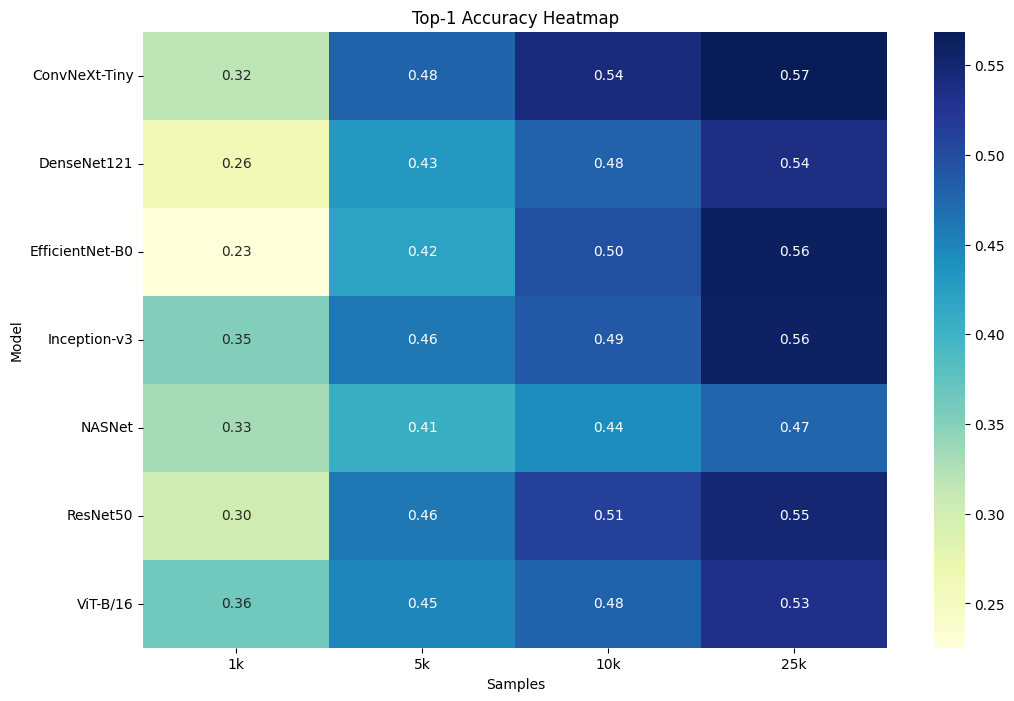
\includegraphics[width=0.8\textwidth]{images/phase03/top-1-heatmap.png}
    \caption{Összehasonlító Top-1 heatmap az iteratív tanításáról.}
    \label{fig:top1_heatmap}
    \end{figure}

    \subsubsection{Összehasonlító precision heatmap az iteratív tanításáról}
    \begin{figure}[H]
    \centering
    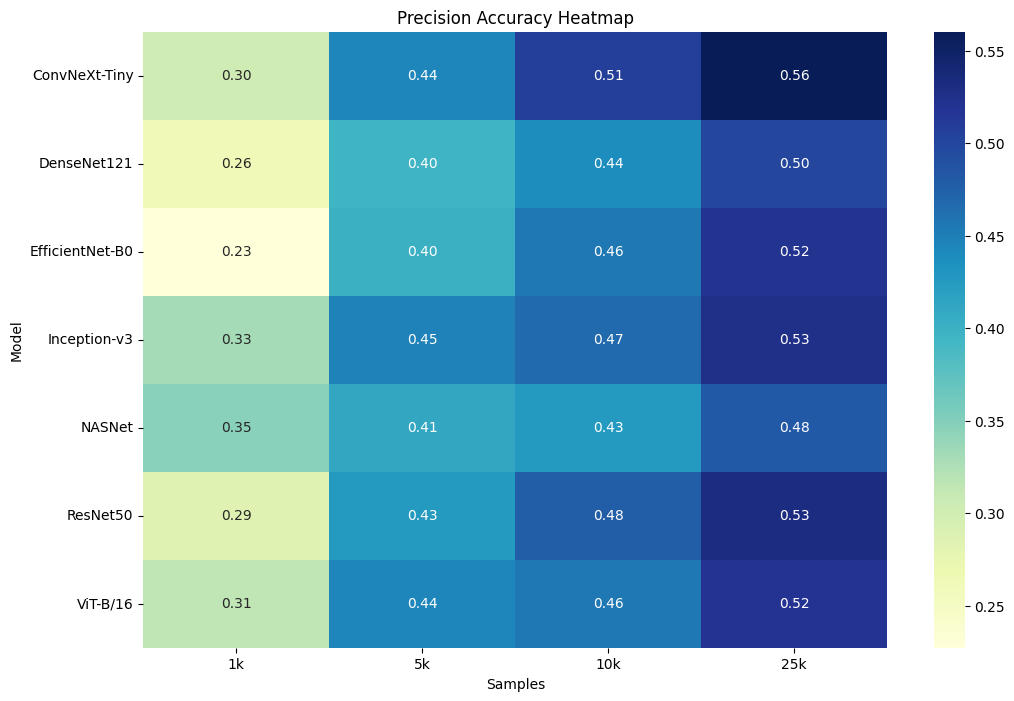
\includegraphics[width=0.8\textwidth]{images/phase03/precision_heatmap.png}
    \caption{Összehasonlító precision heatmap az iteratív tanításáról.}
    \label{fig:precision_heatmap}
    \end{figure}

    \begin{center}
        \begin{longtable}{llllllll}
        \caption{Összehasonlító táblázat az összes modell iteratív tanításáról.}\label{tab:phase4_summary_table}\\
        \toprule
        Modell & Minták & Top-1 & Top-5 & Precision & Recall & F1 & Time(s) \\
        \midrule
        \endfirsthead
        \toprule
        Modell & Minták & Top-1 & Top-5 & Precision & Recall & F1 & Time(s) \\
        \midrule
        \endhead
        ResNet50 & 1k & 0.302 & 0.650 & 0.285 & 0.315 & 0.282 & 31.490 \\
        ResNet50 & 5k & 0.460 & 0.777 & 0.425 & 0.476 & 0.432 & 31.720 \\
        ResNet50 & 10k & 0.513 & 0.818 & 0.478 & 0.542 & 0.490 & 31.710 \\
        ResNet50 & 25k & 0.550 & 0.838 & 0.531 & 0.598 & 0.544 & 31.820 \\
        DenseNet121 & 1k & 0.265 & 0.551 & 0.264 & 0.286 & 0.254 & 25.090 \\
        DenseNet121 & 5k & 0.431 & 0.751 & 0.396 & 0.449 & 0.405 & 24.870 \\
        DenseNet121 & 10k & 0.479 & 0.785 & 0.439 & 0.506 & 0.454 & 25.020 \\
        DenseNet121 & 25k & 0.537 & 0.821 & 0.500 & 0.574 & 0.517 & 24.710 \\
        EfficientNet-B0 & 1k & 0.225 & 0.477 & 0.227 & 0.249 & 0.218 & 24.750 \\
        EfficientNet-B0 & 5k & 0.421 & 0.750 & 0.401 & 0.463 & 0.412 & 24.640 \\
        EfficientNet-B0 & 10k & 0.498 & 0.806 & 0.455 & 0.526 & 0.473 & 24.670 \\
        EfficientNet-B0 & 25k & 0.563 & 0.846 & 0.521 & 0.607 & 0.546 & 24.780 \\
        ConvNeXt-Tiny & 1k & 0.317 & 0.623 & 0.303 & 0.345 & 0.303 & 25.450 \\
        ConvNeXt-Tiny & 5k & 0.478 & 0.794 & 0.444 & 0.490 & 0.452 & 25.450 \\
        ConvNeXt-Tiny & 10k & 0.542 & 0.827 & 0.508 & 0.566 & 0.514 & 25.270 \\
        ConvNeXt-Tiny & 25k & 0.569 & 0.849 & 0.560 & 0.623 & 0.568 & 25.330 \\
        ViT-B/16 & 1k & 0.364 & 0.665 & 0.314 & 0.353 & 0.314 & 41.850 \\
        ViT-B/16 & 5k & 0.448 & 0.733 & 0.444 & 0.480 & 0.436 & 41.930 \\
        ViT-B/16 & 10k & 0.478 & 0.764 & 0.456 & 0.507 & 0.454 & 41.930 \\
        ViT-B/16 & 25k & 0.533 & 0.819 & 0.519 & 0.591 & 0.531 & 42.080 \\
        Inception-v3 & 1k & 0.352 & 0.681 & 0.331 & 0.358 & 0.322 & 33.270 \\
        Inception-v3 & 5k & 0.460 & 0.787 & 0.447 & 0.486 & 0.447 & 33.300 \\
        Inception-v3 & 10k & 0.489 & 0.799 & 0.467 & 0.519 & 0.473 & 33.680 \\
        Inception-v3 & 25k & 0.560 & 0.844 & 0.525 & 0.582 & 0.534 & 33.460 \\
        NASNet & 1k & 0.332 & 0.613 & 0.346 & 0.369 & 0.326 & 81.040 \\
        NASNet & 5k & 0.406 & 0.691 & 0.410 & 0.428 & 0.384 & 81.540 \\
        NASNet & 10k & 0.444 & 0.766 & 0.425 & 0.474 & 0.413 & 81.460 \\
        NASNet & 25k & 0.475 & 0.806 & 0.481 & 0.529 & 0.469 & 81.430 \\
        \bottomrule
        \end{longtable}
    \end{center}
    \cleardoublepage
    
    A különböző képosztályozó modellek iteratív tanítása során egyértelműen kirajzolódik, hogy a mintaszám növelésével minden architektúra esetében fokozatos teljesítményjavulás tapasztalható. Ez jól mutatja a tanítási adathalmaz méretének meghatározó szerepét a hálózatok tanulóképességében és általánosító erejében.
    \\\\
    A ResNet50, mint klasszikus és stabil alapmodell, kiegyensúlyozott fejlődést mutatott: 1 000 mintával még csak 30,2\%-os Top-1 pontosságot ért el, míg 25 000 mintával ez az érték 54,9\%-ra nőtt. A DenseNet121 szintén hasonló mintázatot mutatott, bár teljesítménye némileg elmaradt a ResNet50-től. A NASNet, noha relatív jól szerepelt kis mintaszám mellett, a későbbi fázisokban lassabban fejlődött, és végül alacsonyabb F1-értékkel zárt, miközben a számítási ideje (81 s) lényegesen magasabb maradt.
    \\\\
    A ConvNeXt-Tiny és az EfficientNet-B0 modern architektúrák kiváló skálázódást mutattak: utóbbi különösen 25k mintával ért el kiemelkedő Top-1 pontosságot (56,3\%) és F1-mutatót (54,6\%), miközben megtartotta alacsony számítási igényét (~25 s). A ConvNeXt-Tiny 25k mintával a legjobb F1-értéket érte el (56,8\%), ami kiemelkedő arányosságot jelez a precizitás és a recall között. A ViT-B/16, bár Transformer-alapú modellként magasabb számítási igényt igényelt (~42 s), fokozatos és stabil növekedést mutatott, viszont nem ugrotta meg a legjobb CNN-ek pontosságát. A legkiegyensúlyozottabb teljesítményt az Inception-v3 nyújtotta, amely konzisztensen fejlődött, és 25k mintával 56\%-os Top-1 pontosságot ért el, F1-mutatója pedig elérte az 53,3\%-ot.
    \\\\
    Általánosságban elmondható, hogy minden modell profitált az iteratív tanításból, de a teljesítményük különböző sebességgel és hatékonysággal skálázódott. A modern, könnyű modellek (pl. EfficientNet-B0, ConvNeXt-Tiny) különösen hatékonynak bizonyultak kisebb számítási költség mellett is, míg a ViT és NASNet architektúrák több erőforrást igényeltek, de nem tudtak arányosan jobban teljesíteni. A mért F1-értékek jó képet adnak arról, mennyire tudtak a modellek kiegyensúlyozottan teljesíteni a helyes pozitív felismerések és a teljes visszakeresés aránya között.
    \\\\
    Ezek az eredmények megerősítik, hogy az adatmennyiség növelése kulcsfontosságú, ugyanakkor a modellválasztás – a számítási költségek és a pontosság fényében – szintén meghatározó tényező a gyakorlati alkalmazhatóság szempontjából.

\section{Következtetések a teljes tanítás után kapott eredményekből.}

    \begin{table}[H]
        \centering
        \caption{Teljes tanítás után elért eredmények (Top-1 szerint csökkenő sorrendben)}
        \begin{tabular}{|l|c|c|c|c|c|c|}
        \hline
        \textbf{Modell} & \textbf{Top-1} & \textbf{Top-5} & \textbf{Prec.} & \textbf{Recall} & \textbf{F1} & \textbf{Idő (s)} \\
        \hline
        EfficientNet-B0 & 0.7649 & 0.9421 & 0.7130 & 0.6950 & 0.7001 & 25.26 \\
        NASNet-A-Large & 0.7626 & 0.9470 & 0.7180 & 0.6875 & 0.6955 & 34.03 \\
        ConvNeXt-Tiny & 0.7624 & 0.9357 & 0.7168 & 0.6841 & 0.6947 & 25.67 \\
        ResNet50 & 0.7553 & 0.9351 & 0.7110 & 0.6808 & 0.6908 & 25.11 \\
        Inception-v3 & 0.7518 & 0.9320 & 0.6963 & 0.6787 & 0.6827 & 33.62 \\
        ViT-B/16 & 0.7414 & 0.9257 & 0.6935 & 0.6636 & 0.6730 & 42.40 \\
        DenseNet121 & 0.7400 & 0.9266 & 0.6811 & 0.6680 & 0.6696 & 25.23 \\
        ResNet18 + Baseline & 0.7303 & 0.9099 & 0.6777 & 0.6490 & 0.6568 & 18.54 \\
        ResNet18 + Hybrid v1 & 0.7276 & 0.9074 & 0.6828 & 0.6369 & 0.6536 & 16.13 \\
        ResNet18 + Deep & 0.7247 & 0.9000 & 0.6673 & 0.6336 & 0.6455 & 16.01 \\
        ResNet18 + Hybrid v2 & 0.7236 & 0.9011 & 0.6669 & 0.6391 & 0.6469 & 15.62 \\
        \hline
        \end{tabular}
    \end{table}

    \subsubsection{Teljes tanítás utáni összesítő Top-1 pontosság.}
    \begin{figure}[H]
    \centering
    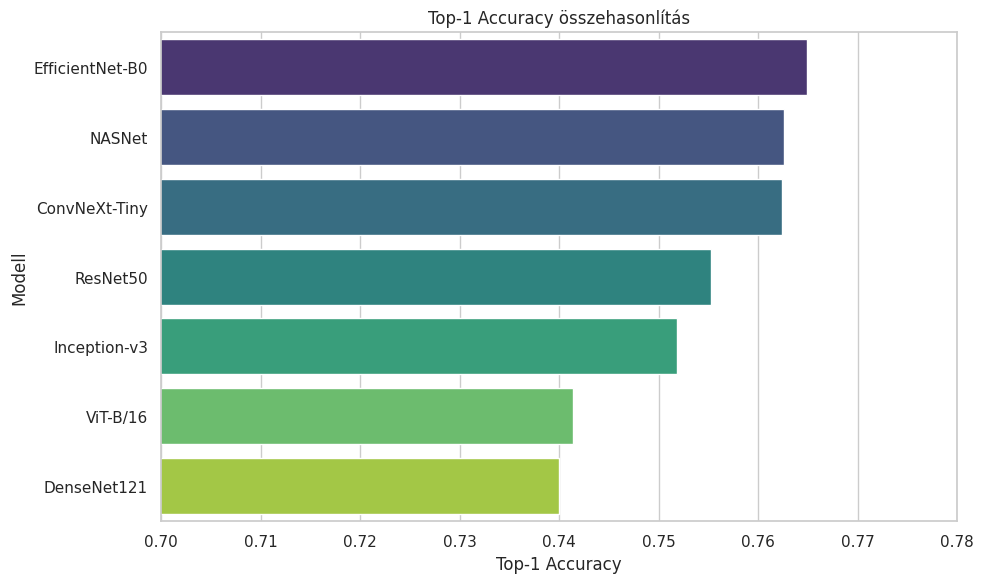
\includegraphics[width=0.7\textwidth]{images/phase02/phase02_summary_top1.png}
    \caption{Teljes tanítás utáni összesítő Top-1 pontosság.}
    \label{fig:phase02_01}
    \end{figure}

    \subsubsection{Teljes tanítás utáni összehasonlító Top-1 és Top-5 pontosság.}
    \begin{figure}[H]
    \centering
    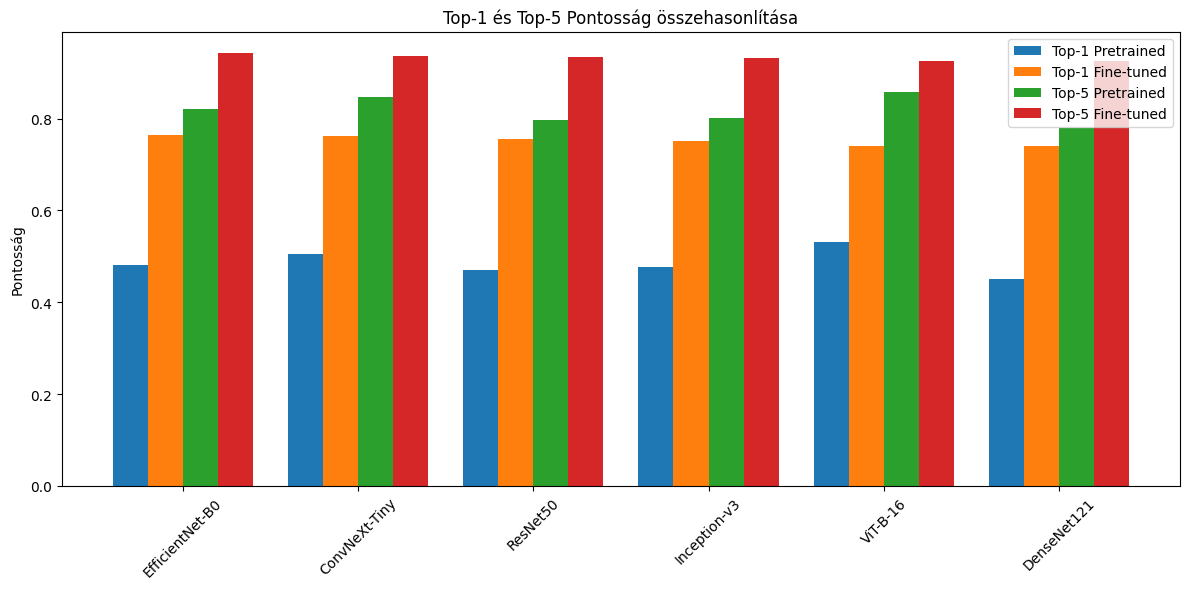
\includegraphics[width=0.7\textwidth]{images/phase02/phase02_summary_top1_vs_top5_pre_vs_fine.png}
    \caption{Teljes tanítás utáni összehasonlító Top-1 és Top-5 pontosság.}
    \label{fig:phase02_02}
    \end{figure}

    \subsubsection{Teljes tanítás utáni összesítő Top-1 pontosság.}
    \begin{figure}[H]
    \centering
    
\includegraphics[width=1.0\textwidth]{images/sum.png}
    \caption{Teljes tanítás utáni összesítő Top-1 pontosság.}
    \label{fig:phase02_03}
    \end{figure}

	A teljes tanítással végzett modellek elemzése alapján több fontos és meglepő megfigyelés is levonható:
	\\\\
    EfficientNet-B0 vezeti a mezőnyt: Bár eredetileg egy kompakt, mobilbarát hálózatként lett tervezve, az EfficientNet-B0 a legmagasabb Top-1 pontosságot (0.7649) és egyben az egyik legjobb F1-score értéket (0.7001) érte el. Ez kiemeli az architekturális hatékonyság és a méretezés szerepét a transfer learning során.
	\\\\
    NASNet-A-Large jelentős javulása: Tanítás nélkül a NASNet alulteljesített (0.2820 Top-1), de tanítással 0.7626 Top-1 pontosságot ért el. Ez azt mutatja, hogy bizonyos hálózatok „alvó potenciállal” rendelkeznek, és megfelelő finomhangolással rendkívül versenyképesek lehetnek.
	\\\\
    Transformer-alapú modellek stabilak, de nem verhetetlenek: A ViT-B/16 transformer modell jó teljesítményt mutatott (0.7414 Top-1), de nem emelkedett ki a többi CNN modell közül. Ez arra utal, hogy nagyobb adattömeg vagy hosszabb tanítási idő szükséges a transzformerek kiemelkedő teljesítményéhez a közepes méretű feladatokon.
	\\\\
    Könnyű fejekkel rendelkező ResNet18-alapú modellek is versenyképesek: A ResNet18 + különböző fejek kombinációja (Baseline, Deep, Hybrid v1/v2) 0.7236–0.7303 Top-1 pontosságot hozott. Ez figyelemre méltó, tekintve az alacsony számítási igényt és egyszerű architektúrát. A Baseline fej valamivel jobb eredményt produkált, mint a Deep vagy Hybrid fejek – valószínűleg az egyszerűbb modell kevésbé hajlamos az overfittingre a futási ideje viszont jelentősen jobb lett, így a Hybrid-v1 versenyképes eggyensúlyt tart a gyorsaság és a pontosság között és felveszi a versenyt a nagy modellekkel.
	\\\\
    Inference idő és teljesítmény kompromisszuma: A ViT és NASNet modellek jelentősen lassabbak (42–275 másodperc!), míg a ResNet18 alapú modellek gyorsak (15–18 másodperc). Ebből adódóan alkalmazás-specifikusan a legjobb választás nem mindig a legpontosabb modell – valós idejű rendszerekhez például egy ResNet18 + Hybrid fej lehet ideális kompromisszum.
	\\\\
    Top-5 pontosság is szoros versenyt mutat: A legtöbb modell 0.90 fölé emelkedett tanítás után, ami azt mutatja, hogy a modellek már nemcsak az első, hanem a legvalószínűbb néhány osztály közé is gyakran eltalálják a helyes címkét. Ez fontos többválaszos vagy javaslat-alapú rendszerek esetén.

\chapter{Összefoglaló}
\label{ch:summary}

A dolgozat célja a fotó osztályozási probléma vizsgálata volt neurális hálózatokkal saját nagyméretű címkézett adatbázison. 
A vizsgálat során összegyűjtöttem 180750 egyedi fotót az elmúlt 20 év saját készítésű képeiből, ebből címkézett adatbázist készítettem SBphotothemes180k néven kétféle címkézéssel.
Az ImageNet1K címkékből 114 kategória adta az első osztályozást a 300 képnél kisebb osztályok megszüntetése után, a Places365 címkékből 121 kategória adta a második osztályozást. Ezek után 80-10-10 arányban felosztottam tanító, validáló és tesztelő adathalmazra az adatbázist. Az adathalmaz képeit 224*244 méretű négyzetes jpg 80 tömörítésű képekké konvertáltam. Így a közel 2TB mennyiségű forrásképből nagyjából 10GB méretű adatbázis készült.
Az elkészült adatbázison vizsgáltam az osztályozási eloszlásokat, és az EXIF adatokat. Az osztályozások estén az átlagos osztályméret 1500 kép körül alakult, a medián 1000 kép körül alakult ami jó, de mivel természetes adatokról beszélünk, így az aszimmetria magas, 8.4 és a szórás is magas 3200 körüli tehát tipikus Long-tail eloszlást mutat.
Az EXIF adatok konverzió közbeni megőrzése és elemzése különösen fontos volt a részletes statisztikák elvégzéséhez és a későbbi vizsgálatok lehetőségeinek biztosításához. 
Az így elkészített adatbázis segítségével három fázisos vizsgálatot végeztem hét ismert és gyakran használt modellen. Ezek a modellek a ResNet50, DenseNet121, EfficientNet-B0, ConvNeXt-Tiny, ViT-B/16, Inception-v3, NASNet voltak. 
Az alkalmazott metrikák a következőek lettek: Top-1 és Top-5 pontosság, Precision, Recall, F1-score. Ezeken túl vizsgáltam a tanítás közbeni validációs és tanítási pontosságokat.
Mindhárom vizsgálatot ugyanazon az teszt adathalmazon végeztem, de más-más tanítóhalmazzal tanítottam. A három vizsgálati fázis a tanítás nélküli tesztelés, majd a teljes tanítás utáni vizsgálat volt, végül az iteratívan növekvő tanítóhalmaz vizsgálata következett. 
A vizsgálat első lépése a tanítás nélküli modellek tesztelése volt a beépített súlyokkal. Ekkor a modellek 50\% körüli Top 1 és 80\% körüli Top 5 pontosságot és 40\% körüli Precision-t nyújtottak. Itt a ConvNeXt-Tiny és ViT-B/16 emelkedtek ki.
A második fázis során a teljes 144000 képes tanítóhalmazon tanítottam minden modellt 10 epoch-on keresztül. Ekkor a modellek 75\% körüli Top 1 és 90\% körüli Top 5 pontosságot és 70\% körüli Precision-t nyújtottak a EfficientNet-B0 és NASNet emelkedtek ki.
Az utolsó vizsgálat során mindig a tanítatlan modellről indulva 1000, 5000, 10000, 25000 képes tanítóhalmazon vizsgáltam a modelleket szintén 10 epoch-on keresztül.
Az adataink alapján a ConvNeXt-Tiny és az EfficientNet-B0 modellek kiemelkedtek 25000 mintaszámmal történő tanítás után, míg a ResNet50 és DenseNet121 modellek gyengébben teljesítettek az alacsonyabb mintaszámokon, de növekvő mintaszámmal jelentős javulást mutattak. Eközben az Inception-v3 és a ViT-B/16 pedig a kis adathalmazon mutatott pontosság terén emelkedtek ki.
Ezután megkíséreltem elkészíteni egy kis méretű, lokális alkalmazásra optimalizált erőforrástakarékos modellt a ResNet18-ra építve egy saját fejrész kifejlesztésével. 
Ennek során 4 modellt készítettem, egy egyrétegű, egy mély, és két modern fejrésszel rendelkezőt. Ezen a négy modellen is elvégeztem a fent ismertetett három mérési fázist. Az egyrétegű fej meglepően jól teljesített, a mély fejrész viszont jelentősen alulmaradt a fenti metrikákban, a modern fejrész csak kicsit nyújtott nagyobb pontosságot, mint az egyrétegű, de jelentősen gyorsabban futott. Összességében a kifejlesztett modell csak kis mértékben maradt alul a vizsgált hatalmas modellektől, de futási teljesítménye sokkal jobb azokénál így nem pontosságkritikus, de erőforráskímélő megoldásokhoz, például hordozható eszközök számára ideális.
Összességében a nagyméretű adathalmaz, a többféle osztályozás, a nagy mennyiségű mért adat és a saját modellek további vizsgálatok alapját képezhetik a jövőben.